%% This is file `sample-manuscript.tex',
%% generated with the docstrip utility.
%%
%% The original source files were:
%%
%% samples.dtx  (with options: `manuscript')
%% 
%% IMPORTANT NOTICE:
%% 
%% For the copyright see the source file.
%% 
%% Any modified versions of this file must be renamed
%% with new filenames distinct from sample-manuscript.tex.
%% 
%% For distribution of the original source see the terms
%% for copying and modification in the file samples.dtx.
%% 
%% This generated file may be distributed as long as the
%% original source files, as listed above, are part of the
%% same distribution. (The sources need not necessarily be
%% in the same archive or directory.)
%%
%% Commands for TeXCount
%TC:macro \cite [option:text,text]
%TC:macro \citep [option:text,text]
%TC:macro \citet [option:text,text]
%TC:envir table 0 1
%TC:envir table* 0 1
%TC:envir tabular [ignore] word
%TC:envir displaymath 0 word
%TC:envir math 0 word
%TC:envir comment 0 0
%%
%%
%% The first command in your LaTeX source must be the \documentclass command.
%%%% Small single column format, used for CIE, CSUR, DTRAP, JACM, JDIQ, JEA, JERIC, JETC, PACMCGIT, TAAS, TACCESS, TACO, TALG, TALLIP (formerly TALIP), TCPS, TDSCI, TEAC, TECS, TELO, THRI, TIIS, TIOT, TISSEC, TIST, TKDD, TMIS, TOCE, TOCHI, TOCL, TOCS, TOCT, TODAES, TODS, TOIS, TOIT, TOMACS, TOMM (formerly TOMCCAP), TOMPECS, TOMS, TOPC, TOPLAS, TOPS, TOS, TOSEM, TOSN, TQC, TRETS, TSAS, TSC, TSLP, TWEB.
% \documentclass[acmsmall]{acmart}

%%%% Large single column format, used for IMWUT, JOCCH, PACMPL, POMACS, TAP, PACMHCI
% \documentclass[acmlarge,screen]{acmart}

%%%% Large double column format, used for TOG
\documentclass[acmtog, authorversion]{acmart}

%%%% Generic manuscript mode, required for submission
%%%% and peer review
%\documentclass[manuscript,screen,review]{acmart}
%% Fonts used in the template cannot be substituted; margin 
%% adjustments are not allowed.
%%
%% \BibTeX command to typeset BibTeX logo in the docs
\AtBeginDocument{%
  \providecommand\BibTeX{{%
    \normalfont B\kern-0.5em{\scshape i\kern-0.25em b}\kern-0.8em\TeX}}}

%% Rights management information.  This information is sent to you
%% when you complete the rights form.  These commands have SAMPLE
%% values in them; it is your responsibility as an author to replace
%% the commands and values with those provided to you when you
%% complete the rights form.
\setcopyright{acmcopyright}
\copyrightyear{2018}
\acmYear{2018}
\acmDOI{XXXXXXX.XXXXXXX}

%% These commands are for a PROCEEDINGS abstract or paper.
\acmConference[Conference acronym 'XX]{Make sure to enter the correct
  conference title from your rights confirmation emai}{June 03--05,
  2018}{Woodstock, NY}
%
%  Uncomment \acmBooktitle if th title of the proceedings is different
%  from ``Proceedings of ...''!
%
\acmBooktitle{Woodstock '18: ACM Symposium on Neural Gaze Detection,
 June 03--05, 2018, Woodstock, NY} 
\acmPrice{15.00}
\acmISBN{978-1-4503-XXXX-X/18/06}


%%
%% Submission ID.
%% Use this when submitting an article to a sponsored event. You'll
%% receive a unique submission ID from the organizers
%% of the event, and this ID should be used as the parameter to this command.
%%\acmSubmissionID{123-A56-BU3}

%%
%% For managing citations, it is recommended to use bibliography
%% files in BibTeX format.
%%
%% You can then either use BibTeX with the ACM-Reference-Format style,
%% or BibLaTeX with the acmnumeric or acmauthoryear sytles, that include
%% support for advanced citation of software artefact from the
%% biblatex-software package, also separately available on CTAN.
%%
%% Look at the sample-*-biblatex.tex files for templates showcasing
%% the biblatex styles.
%%

%%
%% The majority of ACM publications use numbered citations and
%% references.  The command \citestyle{authoryear} switches to the
%% "author year" style.
%%
%% If you are preparing content for an event
%% sponsored by ACM SIGGRAPH, you must use the "author year" style of
%% citations and references.
%% Uncommenting
%% the next command will enable that style.
%%\citestyle{acmauthoryear}

%%
%% end of the preamble, start of the body of the document source.

\usepackage{xcolor}
\usepackage[colorinlistoftodos,prependcaption,textsize=tiny]{todonotes}
\setlength{\marginparwidth}{2.5cm}
\usepackage{algorithm}
\usepackage{algpseudocode}
\usepackage{amsmath}    % For math environments and \text
\usepackage{amssymb}    % For mathematical symbols
\usepackage{bbm}        % For \mathbbm
\usepackage{graphicx}   % For \includegraphics

% Add this in the preamble (after \usepackage declarations)
\newcommand{\redtodo}[1]{\todo[inline, color=red]{\textbf{TODO:} #1}}

\begin{document}

%%
%% The "title" command has an optional parameter,
%% allowing the author to define a "short title" to be used in page headers.

% \title[Tiny Embeddings]{Tiny Embeddings: Leveraging Matryoshka Learning, Quantization, and Bitwise Operations for Reduced Storage and Improved Retrieval Speed}

\title[Quantization Aware Matryoshka Adaptation]{Quantization Aware Matryoshka Adaptation: Leveraging Matryoshka Learning, Quantization, and Bitwise Operations for Reduced Storage and Improved Retrieval Speed}

%%
%% The "author" command and its associated commands are used to define
%% the authors and their affiliations.
%% Of note is the shared affiliation of the first two authors, and the
%% "authornote" and "authornotemark" commands
%% used to denote shared contribution to the research.

%%
%% By default, the full list of authors will be used in the page
%% headers. Often, this list is too long, and will overlap
%% other information printed in the page headers. This command allows
%% the author to define a more concise list
%% of authors' names for this purpose.
%\renewcommand{\shortauthors}{Trovato and Tobin, et al.}

%%
%% The abstract is a short summary of the work to be presented in the
%% article.
\begin{abstract}  
  High-dimensional embeddings are powerful tools in natural language processing and information retrieval, capturing intricate semantic relationships. 
  However, their large size leads to increased storage requirements and slower retrieval speeds, posing challenges for deployment in resource-constrained environments. 
  In this paper, we introduce \textbf{Tiny Embeddings}, a novel approach that combines \textit{Matryoshka Representation Learning}, advanced quantization techniques, and efficient bitwise operations to create compact and efficient embeddings. 
  By augmenting existing models with additional feedforward neural network layers and specialized loss functions, we enforce the Matryoshka property, enabling the use of lower-dimensional embeddings without significant performance loss. 
  We explore 0.5-bit, 1-bit, 1.5-bit, and 2-bit quantization levels to reduce storage by decreasing numeric precision. 
  To further enhance retrieval speed, we extend the use of Hamming distance and similarity to multi-bit quantized embeddings by mapping them to binary representations, allowing efficient computation using bitwise CPU instructions like XOR, NOT, and POPCOUNT. 
  Our hybrid architecture applies higher precision quantization to dimensions with more information content and lower precision to those with less, optimizing storage and performance. 
  Experimental results demonstrate that our approach significantly reduces storage requirements and improves retrieval speeds while maintaining competitive accuracy compared to uncompressed embeddings.  
  
  \end{abstract} 

\begin{abstract}
  We introduce \emph{Quantization Aware Matryoshka Adaptation (QAMA)}, a unified framework for creating compact yet semantically rich embeddings through \textbf{Matryoshka Representation Learning} and multi-level quantization. Our approach learns nested embeddings that gracefully shrink to smaller dimensional subsets and leverages bitwise operations (XOR, NOT, POPCOUNT) for efficient retrieval. By augmenting transformer-based encoders with lightweight feedforward layers and specialized regularization (Matryoshka Loss, Orthogonality, Information Bottleneck, and Quantization Loss), we produce quantization-friendly representations that preserve essential information in early dimensions.

  We explore 0.5-bit, 1-bit, 1.5-bit, and 2-bit quantization levels, as well as a Hybrid Quantization scheme that adaptively allocates higher precision to dimensions with greater information content. Across extensive evaluations on Modern BERT (MB) and MiniLM models, \textbf{2-bit quantization} and \textbf{Hybrid Quant} consistently recover up to 95--98\% of the original full-precision (FP32) performance while reducing memory usage by over 90\%. Even at low embedding dimensions (e.g., 96--192), QAMA’s hierarchical training ensures that performance remains surprisingly robust, highlighting the effectiveness of our bit-level expansions and nested representation learning.

  Furthermore, our experiments show that end-to-end training with quantization-aware losses yields embeddings that map cleanly into discrete levels, supporting rapid Hamming distance calculations for large-scale retrieval. Ablation studies reveal that each component---Matryoshka Loss, Orthogonality, Information Bottleneck, and Adaptive Variance Control---contributes to preserving semantic fidelity under aggressive compression. Overall, \textbf{QAMA} offers a practical means to store and retrieve embeddings efficiently, enabling high-accuracy search under stringent memory and latency constraints.
\end{abstract}

%%
%% The code below is generated by the tool at http://dl.acm.org/ccs.cfm.
%% Please copy and paste the code instead of the example below.
%%
\begin{CCSXML}
<ccs2012>
 <concept>
  <concept_id>10010520.10010553.10010562</concept_id>
  <concept_desc>Computer systems organization~Embedded systems</concept_desc>
  <concept_significance>500</concept_significance>
 </concept>
 <concept>
  <concept_id>10010520.10010575.10010755</concept_id>
  <concept_desc>Computer systems organization~Redundancy</concept_desc>
  <concept_significance>300</concept_significance>
 </concept>
 <concept>
  <concept_id>10010520.10010553.10010554</concept_id>
  <concept_desc>Computer systems organization~Robotics</concept_desc>
  <concept_significance>100</concept_significance>
 </concept>
 <concept>
  <concept_id>10003033.10003083.10003095</concept_id>
  <concept_desc>Networks~Network reliability</concept_desc>
  <concept_significance>100</concept_significance>
 </concept>
</ccs2012>
\end{CCSXML}

\ccsdesc[500]{Computer systems organization~Embedded systems}
\ccsdesc[300]{Computer systems organization~Redundancy}
\ccsdesc{Computer systems organization~Robotics}
\ccsdesc[100]{Networks~Network reliability}

%%
%% Keywords. The author(s) should pick words that accurately describe
%% the work being presented. Separate the keywords with commas.
\keywords{datasets, neural networks, gaze detection, text tagging}

%% A "teaser" image appears between the author and affiliation
%% information and the body of the document, and typically spans the
%% page.

% \begin{teaserfigure}
%   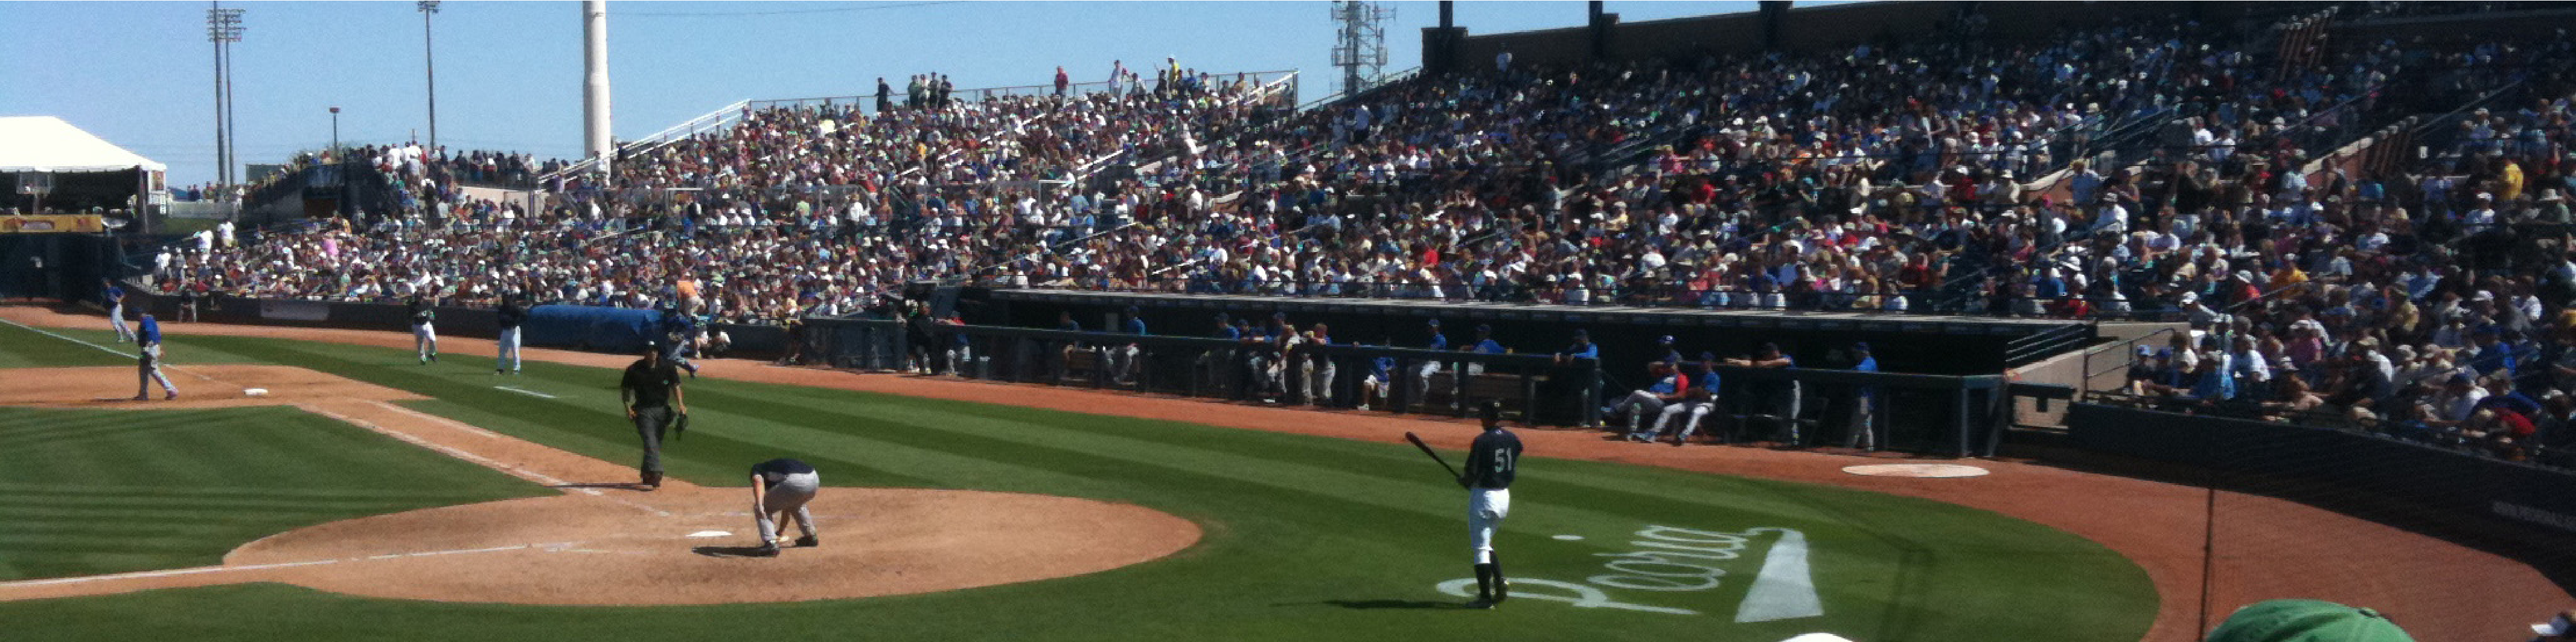
\includegraphics[width=\textwidth]{sampleteaser}
%   \caption{Seattle Mariners at Spring Training, 2010.}
%   \Description{Enjoying the baseball game from the third-base
%   seats. Ichiro Suzuki preparing to bat.}
%   \label{fig:teaser}
% \end{teaserfigure}

%%
%% This command processes the author and affiliation and title
%% information and builds the first part of the formatted document.
\maketitle

\section{Introduction}  
  
In the era of big data and large-scale machine learning applications, efficient representation of textual information is crucial. Embeddings serve as foundational elements in natural language processing (NLP) and information retrieval (IR), transforming text into high-dimensional vectors that capture semantic and syntactic nuances. While high-dimensional embeddings provide rich representations, they come with substantial storage costs and computational overhead, particularly in environments with limited resources or when deploying models to edge devices.  
  
Reducing the size of embeddings without sacrificing performance has become an important research area. Traditional methods such as dimensionality reduction and quantization have been employed, but often at the expense of degrading the quality of embeddings or losing critical information. Optimizing embeddings to be both compact and efficient while retaining high performance remains a significant challenge.  
  
In this paper, we present \textbf{Tiny Embeddings}, an innovative approach that addresses the challenges of storage and retrieval efficiency. Our method leverages \textit{Matryoshka Representation Learning}, named after the Russian nesting dolls, where embeddings of smaller dimensions are nested within larger ones. By adding additional feedforward neural network (FFN) layers and specialized loss functions to existing embedding models, we imbue them with the Matryoshka property. This ensures that essential information is concentrated in the early dimensions, allowing for the use of lower-dimensional embeddings without significant performance degradation.  
  
The \textbf{Matryoshka property} refers to the hierarchical nesting of embeddings, analogous to Russian nesting dolls, where embeddings of smaller dimensions are subsets of larger ones. This property allows for dynamic selection of embedding dimensions based on resource constraints or performance requirements without retraining the model. By concentrating more information in the early dimensions, we enable the use of lower-dimensional embeddings that still capture essential semantic content.  

Furthermore, we introduce trainable quantization techniques, applying 0.5-bit, 1-bit, 1.5-bit, and 2-bit quantization levels to the embeddings. By reducing the numeric precision, we decrease storage requirements substantially. The quantization is made trainable through added FFN layers and loss functions that promote quantization during training.  
  
To enhance retrieval speed, especially on commodity hardware, we propose extending the use of Hamming distance and similarity to multi-bit quantized embeddings. By mapping multi-bit embeddings to higher-bit binary representations (e.g., converting 1.5-bit to 2-bit or 2-bit to 3-bit), we enable efficient computation of similarity using bitwise operations such as XOR, NOT, and POPCOUNT. These operations are highly optimized on modern CPUs, resulting in significantly faster retrieval compared to traditional floating-point calculations used in cosine similarity.  
  
Our hybrid architecture assigns higher precision quantization (e.g., 2-bit) to the early embedding dimensions, which contain more critical information, and lower precision quantization (e.g., 1-bit or 0.5-bit) to later dimensions with less information content. This alignment ensures an optimal balance between storage efficiency and representation quality.  
  
An important insight from our work is that simply selecting embedding dimensions based on variance or gradient importance did not yield satisfactory results. This observation led us to employ Matryoshka representation learning, which effectively concentrates information in early dimensions and overcomes the limitations of naive dimension selection methods.  
  
Our contributions can be summarized as follows:  
  
\begin{enumerate}  
    \item \textbf{Integration of Matryoshka Representation Learning}: We enhance existing embedding models by adding FFN layers and specialized loss functions to enforce the Matryoshka property, empirically demonstrating that addtional FFN layers can learn this property with light weight training without requiring pre-training of full models for this property. This allows the use of fewer embedding dimensions without significant performance loss.
  
    \item \textbf{Trainable Quantization with Multiple Bit Levels}: We introduce trainable quantization techniques using 0.5-bit, 1-bit, 1.5-bit, and 2-bit quantization levels through additional FFN layers and quantization-promoting loss functions, reducing storage requirements by decreasing numeric precision.  
  
    \item \textbf{Novel Quantization Levels}: We explore the application of \textbf{0.5-bit, 1-bit, 1.5-bit, and 2-bit quantization}. By reducing the bits used per dimension, we significantly decrease the storage requirements of the embeddings while controlling the trade-off between compression and performance.  
  
    \item \textbf{Hybrid Quantization Architecture}: We propose a hybrid architecture that applies different quantization levels to different segments of the embedding dimensions, allocating higher precision to dimensions with more information content. Specifically, we use 2-bit quantization for the early \( K \) dimensions, 1.5-bit for the next \( L \) dimensions, 1-bit for the subsequent \( M \) dimensions, and 0.5-bit for the remaining dimensions. This design ensures that dimensions with higher information content receive finer-grained representation, aligning storage precision with the importance of the information captured.
  
    \item \textbf{Efficient Similarity Computation Using Bitwise Operations}: We propose using Hamming distance and Hamming similarity on the bitwise representations of embeddings. For 1.5-bit and 2-bit quantization levels, we map embeddings to higher-bit binary representations (e.g., converting 1.5-bit to 2-bit and 2-bit to 3-bit) to facilitate efficient computation using bitwise operations such as XOR, NOT, and POPCOUNT. This approach improves retrieval speed by leveraging CPU instructions optimized for such operations.  
  
    % \item \textbf{Overcoming Limitations of Dimension Selection/Pruning Methods}: We demonstrate that conventional methods of selecting important embedding dimensions are ineffective, and that Matryoshka learning effectively concentrates information in early dimensions. By integrating Matryoshka learning with embedding quantization, we are able to reduce both the number of embedding dimensions and their precision, leading to compact representations without substantial loss of similarity information.  
  
\end{enumerate}  
simply selecting embedding dimensions based on variance or gradient importance did not yield satisfactory results. This observation underscores the effectiveness of our Matryoshka learning approach, which inherently prioritizes information content in the early dimensions.  
Our experimental evaluations on benchmark datasets demonstrate that Tiny Embeddings achieve significant reductions in storage requirements and retrieval times while maintaining competitive accuracy compared to uncompressed models. The proposed methods offer practical solutions for deploying efficient embeddings in large-scale IR systems and resource-constrained environments.  
  
The remainder of this paper is organized as follows: Section~\ref{sec:related_work} reviews related work on embedding compression and quantization. Section~\ref{sec:methodology} details our proposed methods, including the mathematical formulations of Matryoshka learning and quantization techniques. Section~\ref{sec:experiments} presents the experimental setup and results. Finally, Section~\ref{sec:conclusion} concludes the paper and discusses future research directions.  
  

\section{Related Work}
\label{sec:related_work}

Large-scale language models and high-dimensional embeddings have greatly advanced Natural Language Processing (NLP) and Information Retrieval (IR). 
However, they often demand substantial storage and compute. Various compression techniques have thus emerged to reduce size while retaining performance. 
This section discusses embedding approaches in IR, combined strategies for compressing large language models (LLMs) and embeddings, and Matryoshka Representation Learning (MRL).

\subsection{Embedding Models in Information Retrieval}
Early word embeddings like Word2Vec~\cite{mikolov2013distributed} and GloVe~\cite{pennington2014glove} paved the way for dense vector representations. Subsequent transformers, including BERT~\cite{devlin2019bert}, RoBERTa~\cite{liu2019roberta} and Sentence-BERT~\cite{reimers-2019-sentence-bert}, introduced contextual embeddings with higher accuracy but also higher memory and compute costs. 
Recent research prioritizes compact architectures for deployment efficiency.

\subsection{Compression Techniques for Language Models and Embeddings}
\paragraph{Pruning and Distillation}
\citet{han2015deep} proposed \emph{Deep Compression}, combining pruning, quantization, and coding. The \emph{Lottery Ticket Hypothesis}~\cite{frankle2019lottery} highlights subnetworks that can perform on par with their original dense models. 
Knowledge distillation~\cite{hinton2015distilling, sanh2019distilbert, jiao2020tinybert} transfers capability from large “teacher” models to smaller “student” models.
Recent approaches increasingly integrate compression awareness during training~\cite{shen2021efficient,wang-etal-2024-compression}. 
Our work extends this line by introducing quantization and dimensional hierarchy constraints during the learning phase.


\paragraph{Quantization}
Both post-training~\cite{jacob2018quantization} and quantization-aware training~\cite{hubara2017quantized,mishra2018apprentice} constrain numerical precision. LLM.int8()~\cite{dettmers2022llm} and BitNet~\cite{wang2023bitnet} demonstrate successful quantization for large language models.
Binary and ternary embeddings~\cite{shen2018nash, shu2018compressing} operate efficiently via bitwise operations. 
Product Quantization~\cite{jegou2010product} partitions embeddings into sub-vectors for approximate nearest neighbor search.
Mixed-precision approaches~\cite{dong2019hawq,wang2019haq} allocate different bit-widths based on layer sensitivity. 
In contrast, we propose dimension-wise precision allocation guided by information content

\paragraph{Dimensionality Reduction and Pruning for Embeddings}
Methods like PCA~\cite{jolliffe2016principal}, SVD~\cite{golub1971singular}, and autoencoders~\cite{hinton2006reducing} systematically compress embeddings, while t-SNE~\cite{maaten2008visualizing} and UMAP~\cite{mcinnes2018umap} focus primarily on visualization by preserving local neighborhoods at the expense of global structure and are unsuitable for information retrieval tasks due to their non-parametric nature and inability to process new data without recomputation.
In contrast, our approach creates hierarchical, nested embeddings through explicit loss functions that concentrate essential semantic information in early dimensions while maintaining cross-scale consistency, enabling dynamic dimension selection without retraining and preserving both local and global relationships crucial for retrieval tasks. 
Pruning low-variance dimensions~\cite{li2016pruning} can yield more compact models with minimal loss in semantic fidelity, but lacks the systematic information organization and quantization awareness of our approach.

\paragraph{Efficient Similarity Computation}
Recent advances in approximate nearest neighbor search have leveraged binary codes~\cite{wang2017survey} and locality-sensitive hashing~\cite{andoni2006near, andoni2014beyond}. 
Our work contributes novel bit-level expansions (e.g., 2-bit to 3-bit mapping) that preserve fine-grained similarities while enabling efficient XOR and POPCOUNT operations. 
This bridges the gap between ultra-low-bit quantization and accurate similarity preservation.

\subsection{Matryoshka Representation Learning}
Matryoshka Representation Learning (MRL)~\cite{kusupati2021matryoshka} aims to create hierarchical embeddings where smaller embeddings are nested within larger ones, analogous to Russian nesting dolls. 
This approach allows models to adaptively use embeddings of different sizes based on resource constraints, without the need for retraining. 
MRL focuses on generating these hierarchical embeddings such that truncated dimensions can still yield functional representations. 
While prior works have attempted to promote such nesting properties, they typically did so without explicit loss functions tailored to enforce them.
We incorporate three explicit \emph{Losses to Promote Matryoshka Property} to concentrate key information in early dimensions. 

\subsection{Our Approach in Context}
% We unify MRL with finer-grained quantization and bitwise operations for efficient storage and retrieval. 
% Unlike previous MRL methods, we incorporate three explicit \emph{Losses to Promote Matryoshka Property} to concentrate key information in early dimensions. 
% We also use a hybrid quantization scheme assigning varying bit-levels to embedding slices, balancing performance and storage for diverse IR scenarios.

% Our framework QAMA unifies these directions, introducing three key innovations: (1) quantization-aware Matryoshka learning, (2) hybrid precision allocation, and (3) efficient bit-wise similarity computation. The following section details our technical approach.



While these prior approaches have made significant advances in embedding compression and efficient retrieval, they typically address individual aspects of the problem in isolation. 
Post-training quantization methods~\cite{jacob2018quantization} often struggle with accuracy degradation, while MRL~\cite{kusupati2021matryoshka} lacks explicit mechanisms for ultra-low-bit representations. 
Similarly, current mixed-precision techniques~\cite{dong2019hawq} focus on layer-wise quantization rather than dimension-wise precision allocation that aligns with semantic importance. More recent approaches within Hugging Face, Jina AI and Vespa AI \cite{hf2024quantization, vespa2024matryoshka, jina2024binary} have also focused on MRL and quantization, where \cite{vespa2024matryoshka} has proposed to integrate MRL with quantization, but their training process doesn't adapt older models and doesn't support hybrid precision allocation.

Our framework QAMA unifies and extends these directions through three key innovations:
\begin{enumerate}
    \item \textbf{Quantization-aware Matryoshka Learning:} Unlike previous MRL approaches that focus solely on dimensional hierarchy, we jointly optimize for both nested structure and quantization-friendly representations through specialized loss functions and learned transformations.
    
    \item \textbf{Hybrid Precision Allocation:} We introduce a novel dimension-wise precision scheme that assigns different bit-widths (0.5-bit to 2-bit) based on information content, moving beyond traditional uniform or layer-wise quantization approaches to achieve better compression-accuracy trade-offs.
    
    \item \textbf{Efficient Bit-wise Similarity Computation:} We bridge the gap between ultra-low-bit quantization and accurate similarity preservation through carefully designed bit-level expansions, enabling fast retrieval via hardware-accelerated operations while maintaining fine-grained semantic distinctions.
\end{enumerate}

The following section details our technical approach, describing how these innovations work together to create a unified framework for compact, efficient, and accurate embedding systems.

  
  
\section{Methodology}
\label{sec:methodology}

\subsection{Overview}
Our approach combines multiple techniques to create efficient and compact embeddings while preserving semantic relationships. The key components include:
\begin{itemize}
    \item Neural transformation layers for improved quantization and matryoshka representation learning
    \item Hybrid architecture combining different quantization levels
    \item Loss functions to promote quantization and matryoshka representation learning
    \item Efficient bit-packing and similarity computation
\end{itemize}

\begin{figure}[h]
    \centering
    %\includegraphics[width=\linewidth]{figures/system_architecture.pdf}
    \caption{Overall architecture of Tiny Embeddings system showing the transformation, quantization, and bit-packing stages.}
    \label{fig:system_architecture}
\end{figure}


\subsection{Quantization Framework}
\label{subsec:quantization_framework}

Our quantization framework converts high-precision embeddings into compact, discrete representations while preserving semantic relationships through a combination of neural transformations and adaptive threshold-based discretization. We first apply a feedforward transformation $\mathbf{z} = \text{FFN}(\mathbf{x}; \theta)$ to optimize the embedding space for quantization, where $\mathbf{x}$ is the input embedding and $\theta$ represents trainable parameters.

\paragraph{Multi-level Quantization}
We implement multiple quantization levels for flexible storage-performance trade-offs: 2-bit (4 levels), 1.5-bit (3 levels), 1-bit (2 levels), and 0.5-bit (combines dimension pairs) quantization. For $k$-bit quantization with $2^k$ levels, we use $(2^k - 1)$ learnable thresholds per dimension to partition the continuous embedding space. For instance, 2-bit quantization employs three thresholds $\{\theta_1, \theta_2, \theta_3\}$ to create four bins, while 1-bit quantization uses a single threshold for binary partitioning.

\paragraph{Threshold-based Discretization and Learning}
For a $d$-dimensional embedding space $\mathbf{X} \in \mathbb{R}^{N \times d}$, we initialize thresholds using percentile statistics to ensure balanced quantization:
\begin{equation}
    \theta_{i,j} = \text{Quantile}\bigl(\{x_{1,j}, \ldots, x_{N,j}\},\; q_i\bigr)
\end{equation}
where $q_i$ are evenly-spaced quantiles in $(0,1)$. During training, thresholds adapt via exponential moving average:
\begin{equation}
    \theta_{i,j}^{(\text{new})} = \mu\,\theta_{i,j}^{(\text{old})} + (1-\mu)\;\widehat{\theta}_{i,j}^{(\text{batch})}
\end{equation}
with momentum coefficient $\mu \in [0,1]$ and batch-computed thresholds $\widehat{\theta}_{i,j}^{(\text{batch})}$.

\paragraph{Quantization Process}
The complete process for an input embedding involves: (1) applying the trainable transformation $\mathbf{z} = \text{FFN}(\mathbf{x})$, (2) normalizing $\hat{\mathbf{z}} = \text{normalize}(\mathbf{z})$, and (3) assigning discrete codes:
\begin{equation}
    q_j = \sum_{i=1}^{2^k-1} \mathbbm{1}[\hat{z}_j > \theta_{i,j}]
\end{equation}

\paragraph{End-to-End Trainability}
Our framework achieves end-to-end trainability by optimizing continuous-valued embeddings while simultaneously guiding them toward quantization-friendly distributions. Rather than backpropagating through non-differentiable quantization operations, we apply quantization regularization losses (Section~\ref{subsubsec:quant_reg}) that encourage embeddings to cluster away from quantization boundaries. 
The thresholds themselves are updated using statistics from the continuous embeddings, ensuring the quantization boundaries evolve to match the learned representation space, while the transformation network learns to produce embeddings that naturally align with discrete quantization levels, enabling training without direct gradients through the discretization step.
% This framework offers several advantages: optimal organization of embedding dimensions through learned transformations, balanced quantization bins via adaptive thresholds, flexible storage-performance trade-offs through multiple quantization levels, and end-to-end trainability. 
Experimental results (Section~\ref{sec:experiments}) demonstrate significant compression while maintaining high retrieval accuracy across diverse tasks.







\subsection{Promoting Information High Density in Early Dimensions}
\label{subsec:matryoshka_and_control}
Matryoshka Representation Learning (MRL), inspired by Russian nesting dolls, addresses a fundamental challenge in embedding systems: creating representations that remain effective when truncated to smaller dimensions. Traditional embeddings often lose critical information when dimensions are removed since important features are distributed across all dimensions. Our approach extends MRL with additional control mechanisms to create highly efficient, nested representations where the most crucial information is concentrated in early dimensions.

\subsubsection{Core Matryoshka Architecture}

\paragraph{Nested Representation Generation}
Given an input embedding $\mathbf{x} \in \mathbb{R}^d$, we generate a series of nested representations at different dimension levels $D = \{d_1, d_2, ..., d_K\}$ where $d_1 < d_2 < ... < d_K = d$. Each level $k$ contains all information from previous levels plus additional features:

\begin{equation}
    \mathbf{y}_k = f_k(\mathbf{x}) \in \mathbb{R}^{d_k}, \quad k = 1,\ldots,K
\end{equation}

The key nesting property ensures that smaller representations are perfect subsets of larger ones:
\begin{equation}
    \mathbf{y}_i[1:d_j] = \mathbf{y}_j \quad \text{for } j < i
\end{equation}

\paragraph{Base Transformation Network}
We implement the transformation function $f_k$ using the same lightweight yet effective feed-forward network as introduced in the quantization framework, where $\mathbf{h} = \text{FFN}(\mathbf{x}) = W_2(\text{GELU}(W_1\mathbf{x}))$. Here, $W_1 \in \mathbb{R}^{32d \times d}$ expands the representation for richer feature extraction, GELU activation adds non-linearity while maintaining smooth gradients, and $W_2 \in \mathbb{R}^{d \times 32d}$ projects back to original dimension space. This shared architecture ensures consistency across both the matryoshka representation learning and quantization stages of our pipeline.

\paragraph{Progressive Dimension Slicing}
Unlike traditional MRL implementations that use separate projections for each scale, we employ an efficient progressive slicing mechanism:

\begin{equation}
    \mathbf{y}_k = \text{Slice}_{d_{k-1}}^{d_k}(\mathbf{h})
\end{equation}

The full embedding at level $k$ is constructed through concatenation:
\begin{equation}
    \mathbf{e}_k = [\mathbf{y}_1; \mathbf{y}_2; ...; \mathbf{y}_k]
\end{equation}

This approach inherently maintains the nested property without requiring explicit constraints, reducing computational overhead.

\paragraph{Combined Loss Function}
Our training objective combines multiple loss components, each with their corresponding weights, applied at each dimension level:

\begin{equation}
\begin{split}
    \mathcal{L}_{\text{total}} = & \sum_{d \in D} \sum_{l \in \mathcal{L}} w_l^{(d)} \mathcal{L}_l^{(d)}
\end{split}
\end{equation}

where $w_l^{(d)}$ represents the weight for loss component $l$ at dimension level $d$.

\subsection{Loss Functions and Training Objectives}

In our proposed Matryoshka Representation Learning (MRL) framework, we integrate both \emph{similarity preservation} and \emph{matryoshka adaptation} losses to achieve nested, multilevel embeddings that maintain semantic quality at each quantization level. Additionally, a \emph{quantization regularization} component ensures that the learned representation is readily quantizable with minimal loss in accuracy. Below, we detail each category of losses and explain how they contribute to our overall training scheme.

\subsubsection{Similarity Preservation}

\paragraph{Direct Similarity MSE Loss}
We first ensure preservation of pairwise similarities via a mean squared error (MSE) loss on the normalized similarity matrices:
\begin{equation}
    \mathcal{L}_{\text{sim}}(\mathbf{X}, \mathbf{Y}) = \|\mathbf{S}_X - \mathbf{S}_Y\|_F^2
\end{equation}
where:
\begin{equation}
    \mathbf{S}_X = \text{normalize}(\mathbf{X}) \,\text{normalize}(\mathbf{X})^T, 
    \quad 
    \mathbf{S}_Y = \text{normalize}(\mathbf{Y}) \,\text{normalize}(\mathbf{Y})^T,
\end{equation}
preserving the cosine similarities between all pairs of embeddings $\mathbf{X}$ and $\mathbf{Y}$ at different quantization levels.

\paragraph{KL Divergence Loss}
To align the probability distributions of similarities, we employ a symmetric KL divergence with temperature scaling:
\begin{equation}
    \mathbf{P}_X = \text{softmax}(\mathbf{S}_X/\tau), 
    \quad 
    \mathbf{P}_Y = \text{softmax}(\mathbf{S}_Y/\tau),
\end{equation}
\begin{equation}
    \mathcal{L}_{\text{kl}} = \tfrac{1}{2}\bigl[D_{\text{KL}}(\mathbf{P}_X\|\mathbf{P}_Y) + D_{\text{KL}}(\mathbf{P}_Y\|\mathbf{P}_X)\bigr],
\end{equation}
where $\tau$ controls the sharpness of the distribution.

\paragraph{Rank Preservation Loss}
To maintain the \emph{relative ordering} of similarities, we implement a differentiable ranking loss:
\begin{equation}
    \mathcal{L}_{\text{rank}} = \sum_{i,j,k} \sigma \bigl((s_{ij}^X - s_{ik}^X)\cdot t\bigr) 
    \,\odot\, 
    \sigma \bigl((s_{ij}^Y - s_{ik}^Y)\cdot t\bigr),
\end{equation}
where $\sigma(\cdot)$ is the sigmoid function, $t$ sharpens the sigmoid, and $s_{ij}^X, s_{ij}^Y$ denote pairwise similarities in the original and quantized embeddings respectively.

\paragraph{Contrastive Learning}
We also incorporate contrastive losses with positive and negative pairs:
\begin{equation}
    \mathcal{L}_{\text{contrast}} = -\log\frac{\exp(s_p/\tau)}{\exp(s_p/\tau) + \sum_{n}\exp(s_n/\tau)},
\end{equation}
where $s_p$ and $s_n$ represent the similarities for positive and negative pairs, respectively.

\subsubsection{Losses to Promote Matryoshka Property}
\label{subsubsec:adv_info_control}
To further support the \emph{Matryoshka} property (i.e., nested and progressively expanding embeddings), we introduce three \emph{matryoshka adaptation} losses that manipulate the distribution and uniqueness of information at each dimension level.

\paragraph{Progressive Information Bottleneck}
We encourage essential features to concentrate in earlier dimensions:
\begin{equation}
    \mathcal{L}_{\text{ib}} = \sum_{i=1}^{n} w_i 
    \left(\frac{|\mathbf{x}_i|^2}{x_0 + |\mathbf{x}_i|}\right)^\alpha,
\end{equation}
where $w_i = i/n$ progressively increases with dimension index $i$, $x_0 \approx 0.1$ is a small suppression threshold, and $\alpha\approx 0.3$ controls the gradient strength near zero. This approach pushes less important information toward zero in higher dimensions.

\paragraph{Inter-level Orthogonal Information Encoding}
We promote uniqueness of newly added dimensions by enforcing orthogonality with respect to previously formed dimensions:
\begin{equation}
    \mathcal{L}_{\text{orth}} = \sum_{l=2}^{L} \sum_{j=1}^{l-1} \|\mathbf{\Delta}_l^T \cdot \text{normalize}(\mathbf{E}_j)\|_F,
\end{equation}
where $\mathbf{\Delta}_l$ indicates the newly added dimensions at level $l$, and $\mathbf{E}_j$ consists of all dimensions up to level $j$. This encourages each new level of dimensions to encode novel information rather than rediscovering existing patterns.

\paragraph{Adaptive Variance Control}
To prevent embedding collapse while allowing selective dimension suppression, we employ a slowly increasing variance penalty:
\begin{equation}
    \mathcal{L}_{\text{var}}(t) 
    = 
    \max\Bigl(0.2,\, \frac{e^{t/T} - 1}{e - 1}\Bigr) 
    \sum_{d=1}^D 
    \exp(-\sigma_d),
\end{equation}
where $t$ is the current training step, $T$ is the total training steps, and $\sigma_d$ is the standard deviation of dimension $d$. This loss starts with a weak penalty and grows over time, preventing early collapse and encouraging dimensions that truly matter to preserve sufficient variance.

\subsubsection{Quantization Regularization Loss}
\label{subsubsec:quant_reg}
While the above mechanisms reinforce nested representation properties, we also require a loss term to facilitate \emph{quantization readiness}. This term discourages embeddings from clustering near quantization thresholds and encourages them to lie closer to valid quantized levels.

\paragraph{Formulation}
Let $\theta$ be a quantization threshold for 1-bit quantization, or $\{\theta_1, \theta_2, \theta_3\}$ be thresholds for 2-bit quantization. Denoting each embedding value as $x$, our quantization regularization can be written as:
\begin{equation}
    \mathcal{L}_{\text{quant}} 
    = 
    w(t) 
    \Bigl[
        \exp\bigl(-(\min_i |x - \theta_i|)\bigr) 
        + 
        \lambda\,L_{\text{range}}(x)
    \Bigr],
\end{equation}
where $w(t)$ progresses from $0.2$ to $1.0$ over training to gradually strengthen quantization constraints, and $L_{\text{range}}(x)$ enforces that $x$ lies within a valid range (e.g., $[0,1]$ or another permissible interval). Specifically,
\begin{equation}
    L_{\text{range}}(x) 
    = 
    \text{ReLU}(l - x)^2 
    + 
    \text{ReLU}(x - u)^2,
\end{equation}
where $l$ and $u$ are the lower and upper bounds of acceptable ranges. Intuitively, this loss repels the embedding away from threshold boundaries (to avoid ambiguity) and adjusts overly large or negative values back into a valid quantization domain.


By combining these losses, we achieve a robust training procedure that satisfies several objectives simultaneously:
\begin{itemize}
    \item \textbf{Similarity Preservation:} $\mathcal{L}_{\text{sim}}, \mathcal{L}_{\text{kl}}, \mathcal{L}_{\text{rank}}, \mathcal{L}_{\text{contrast}}$ ensure semantic fidelity across different quantization levels.
    \item \textbf{Matryoshka Property:} $\mathcal{L}_{\text{ib}}, \mathcal{L}_{\text{orth}}, \mathcal{L}_{\text{var}}$ organize the learned features hierarchically, pushing essential features into early dimensions while maintaining uniqueness and stable variance distribution across expanding dimensional levels.
    \item \textbf{Quantization Readiness:} $\mathcal{L}_{\text{quant}}$ directly encourages embeddings to settle into regions that are easily separable by the quantizer, thereby reducing errors from threshold-based discretization.
\end{itemize}

Finally, these losses can be summed with appropriate weights to form the complete training objective.
This unified framework delivers \emph{nested, increasingly robust} embeddings within a single training pipeline, enabling flexible deployment scenarios where early dimensions provide quick approximate search, while further dimensions refine accuracy for more demanding tasks.

\subsection{Hybrid Architecture}
\label{subsec:hybrid_architecture}

We employ a hierarchical scheme that applies different quantization levels to different fractions of the embedding dimensions based on their information content:

\begin{itemize}
    \item \textbf{First 25\% (highest information):} 2-bit quantization (expanded to 3-bit codes) 
    \item \textbf{Next 25\% (medium-high):} 1.5-bit quantization (3 levels, expanded to 2-bit codes) 
    \item \textbf{Next 25\% (medium-low):} 1-bit quantization (direct binary) 
    \item \textbf{Final 25\% (lowest):} 0.5-bit quantization (pairs of dimensions reduced via a lightweight FFN)
\end{itemize}

This arrangement yields an average of 1.625 bits per dimension, balancing storage efficiency and similarity preservation by granting higher precision to dimensions with greater semantic importance.

\paragraph{Dimension Reduction for 0.5-bit Encoding}
For the last quarter of dimensions, pairs are combined:
\begin{equation}
    \mathbf{z}_{\text{reduced}} = \text{FFN}_{\text{reduce}}\Bigl([\mathbf{x}_{2i}, \mathbf{x}_{2i+1}]\Bigr),
\end{equation}
where a specialized FFN preserves essential information while halving the dimensional load. Figure~\ref{fig:hybrid_architecture} illustrates the full hybrid quantization pipeline.

\subsection{Efficient Storage and Similarity Computation}
\label{subsec:storage_and_similarity}

We combine bit-level optimizations with carefully designed expansions that preserve semantic similarity in quantized embeddings while minimizing storage overhead.

\subsubsection{Bit Packing and Storage}
\paragraph{Bit Packing Process:}
\begin{enumerate}
    \item Convert quantized vectors to binary form. 
    \item Pack bits into $N$-bit words ($N \in \{8,16,32\}$) via:
    \begin{equation}
        \mathbf{w}_i = \sum_{j=0}^{N-1} b_{Ni+j} \cdot 2^{N-j-1},
    \end{equation}
    where $b_k$ is the $k$-th bit.
    \item Add padding bits if needed.
    \item Store as \texttt{uint64} arrays for optimal alignment.
\end{enumerate}

\subsubsection{Binary Codebook Expansion}
\paragraph{2-bit to 3-bit:}
\begin{equation}
\text{Codebook}_{2\rightarrow3} =
\begin{cases}
0 \rightarrow [0,0,0]\\
1 \rightarrow [0,0,1]\\
2 \rightarrow [0,1,1]\\
3 \rightarrow [1,1,1]
\end{cases}
\end{equation}
Expanding 2-bit values (0--3) to 3 bits preserves relative distances more accurately, preventing similar embeddings from collapsing to identical Hamming codes.
For example:
\begin{itemize}
    \item Original 2-bit values [0,1] and [1,0] have equal Hamming distance to [1,1]
    \item Expanded codes [0,0,1] and [0,1,1] have different Hamming distances to [1,1,1]
    \item This better reflects the original quantization levels' relationships
\end{itemize}

\paragraph{1.5-bit to 2-bit:}
\begin{equation}
\text{Codebook}_{1.5\rightarrow2} =
\begin{cases}
0 \rightarrow [0,0]\\
1 \rightarrow [0,1]\\
2 \rightarrow [1,1]
\end{cases}
\end{equation}
Maps three-level codes to 2 bits, improving similarity preservation while keeping compact storage.

\subsubsection{Hamming Similarity Computation}
\paragraph{Basic Hamming Similarity:}
For binary vectors $\mathbf{x}, \mathbf{y}$ of length $n$ (bits),
\begin{equation}
    \text{sim}_H(\mathbf{x}, \mathbf{y}) 
    = 
    1 - \frac{\text{POPCOUNT}(\mathbf{x} \oplus \mathbf{y})}{n},
\end{equation}
where $\oplus$ is XOR and \text{POPCOUNT} counts set bits.

\paragraph{Implementation Details:} 
Modern CPUs offer hardware-accelerated \texttt{XOR} and \texttt{POPCNT} instructions (optionally AVX-512) enabling high-throughput Hamming distance computation on packed 64-bit words.
We leverage \texttt{numpy.packbits}, \texttt{numpy.unpackbits}, \texttt{numpy.bitwise\_xor}, and \texttt{numpy.bitwise\_count} for fast, vectorized bit manipulation and codebook expansions.
These strategies tightly pack quantized representations, expand codes to preserve fine-grained similarities, and compute large-scale Hamming distances rapidly, yielding an efficient, similarity-aware embedding system.
\section{Experimental Setup}
\label{sec:experiments}

We evaluated our approach using a suite of benchmark retrieval datasets from the MTEB (Massive Text Embedding Benchmark) library~\cite{muennighoff2022mteb}, including ArguAna~\cite{wachsmuth-etal-2018-retrieval, thakur2021beir}, CQADupstackTexRetrieval~\cite{hoogeveen2015cqadupstack}, ClimateFEVER~\cite{diggelmann2020climatefever}, DBPedia~\cite{hasibi2017dbpedia}, FEVER~\cite{thorne2018fever}, FiQA2018~\cite{thakur2021beir}, HotpotQA~\cite{yang2018hotpotqa}, MSMARCO~\cite{nguyen2016ms}, NFCorpus~\cite{boteva2016full}, NQ (Natural Questions)~\cite{kwiatkowski2019natural}, QuoraRetrieval~\cite{iyer2017first, thakur2021beir}, SCIDOCS~\cite{specter2020cohan}, SciFact~\cite{wadden2020fact}, TREC-COVID~\cite{voorhees2021trec, thakur2021beir}, and Touche2020~\cite{bondarenko2020overview}.


For our experiments, we employed two distinct Transformer models: MiniLM~\cite{minilm, reimers-2019-sentence-bert}, a compact 12-layer model with 384-dimensional embeddings derived through knowledge distillation, and Modern BERT (MB)~\cite{modernbert, nussbaum2024nomic}, a more recent 22-layer architecture with 768-dimensional embeddings incorporating state-of-the-art design principles. This selection allows us to evaluate our approach across different model scales and architectural generations, from efficient distilled models to modern high-capacity architectures.
Demonstrating robust results on both a smaller, older architecture and a more recent, higher-capacity model indicates that practitioners can attain substantial compression benefits—via quantization and nested dimensionality reduction—across diverse Transformer-based architectures.


We compared our approach against the following baselines: \textbf{Original Model (FP32)} (full-precision 32-bit floating point embeddings), \textbf{FP16} (half-precision 16-bit), \textbf{Int8} (8-bit integer quantization), and \textbf{Simple Threshold Quantization} (basic 2-bit, 1.5-bit, and 1-bit quantization using fixed thresholds without learned transformations or Matryoshka representation).

The training process optimizes our Matryoshka model $\mathcal{M}$ initialized from a pretrained model $\mathcal{E}$. 
For each batch, normalized base embeddings are transformed to produce both non-quantized and quantized representations at different dimension levels. 
The training objective combines multiple weighted loss terms: similarity preservation losses ($\mathcal{L}_{\text{sim}}$, $\mathcal{L}_{\text{kl}}$, $\mathcal{L}_{\text{rank}}$, $\mathcal{L}_{\text{contrast}}$), orthogonality loss for unique information across levels, information bottleneck loss to concentrate important features early, and quantization loss to facilitate discretization. 
Quantization thresholds are initialized using percentile-based statistics and updated with momentum. We used AdamW optimizer with $\eta = 1 \times 10^{-4}$, warm-up scheduling, and gradient clipping, training for 5 epochs. 
For evaluation, we used NDCG@10 which measures ranking quality by comparing the relevance scores of retrieved documents against an ideal ranking, normalized to [0,1].

\section{Results and Analysis}
\label{sec:results}

In this section, we present the experimental results of our proposed QAMA (Quantization Aware Matryoshka Adaptation) approach using two different models: Modern BERT (MB) \cite{modernbert, nussbaum2024nomic} and MiniLM \cite{minilm, reimers-2019-sentence-bert}. We evaluate the performance across various embedding dimensions and quantization levels to demonstrate the effectiveness of our methods in reducing storage requirements and improving retrieval speed while maintaining high accuracy.

\subsection{Main Results}

Tables~\ref{tab:mb_main_results} and~\ref{tab:minilm_main_results} provide the performance comparison of the models with different quantization levels and embedding dimensions. The performance metric used is the average nDCG@10 across multiple datasets, including ArguAna, NFCorpus, SCIDOCS, SciFact, and TREC-COVID.

\begin{table}[ht]
\caption{Performance of Modern BERT (MB) with different quantization levels and embedding dimensions.}
\label{tab:mb_main_results}
\centering
\begin{tabular}{lccccc}
\toprule
\textbf{Dimension} & \textbf{1-bit} & \textbf{1.5-bit} & \textbf{Hybrid Quant} & \textbf{2-bit} & \textbf{FP32} \\
\midrule
768 & 0.4381 & 0.4536 & 0.4680 & 0.4687 & 0.4720 \\
384 & 0.4167 & 0.4429 & 0.4509 & 0.4593 & 0.4695 \\
256 & 0.3691 & 0.4228 & 0.4465 & 0.4513 & 0.4680 \\
192 & 0.3285 & 0.3901 & 0.4245 & 0.4327 & 0.4512 \\
96 & 0.2908 & 0.3455 & 0.3850 & 0.3919 & 0.4247 \\
\bottomrule
\end{tabular}
\end{table}

\begin{table}[ht]
\caption{Performance of MiniLM with different quantization levels and embedding dimensions.}
\label{tab:minilm_main_results}
\centering
\begin{tabular}{lccccc}
\toprule
\textbf{Dimension} & \textbf{1-bit} & \textbf{1.5-bit} & \textbf{Hybrid Quant} & \textbf{2-bit} & \textbf{FP32} \\
\midrule
384 & 0.3839 & 0.4101 & 0.4160 & 0.4185 & 0.4286 \\
192 & 0.3724 & 0.3923 & 0.4017 & 0.4109 & 0.4219 \\
128 & 0.3571 & 0.3814 & 0.3865 & 0.3917 & 0.3963 \\
96 & 0.3417 & 0.3649 & 0.3695 & 0.3712 & 0.3792 \\
48 & 0.2687 & 0.2871 & 0.2919 & 0.2897 & 0.3014 \\
\bottomrule
\end{tabular}
\end{table}

From the results, we observe that our proposed Tiny Embeddings achieve competitive performance compared to the full-precision (FP32) embeddings, even at significantly reduced storage sizes. For instance, the 2-bit quantized embeddings at 384 dimensions achieve an nDCG@10 of 0.4593 with MB and 0.4185 with MiniLM, which is close to the FP32 performance while reducing the storage requirements substantially.

\subsection{Impact of Quantization Levels}

We further analyze the impact of different quantization levels on the performance. Figures~\ref{fig:quantization_impact_mb} and~\ref{fig:quantization_impact_minilm} illustrate the performance across different quantization levels for MB and MiniLM models, respectively.

\begin{figure}[ht]
    \centering
    % \includegraphics[width=0.8\linewidth]{figures/quantization_impact_mb.pdf}
    \caption{Impact of quantization levels on performance for Modern BERT (MB) model across different dimensions.}
    \label{fig:quantization_impact_mb}
\end{figure}

\begin{figure}[ht]
    \centering
    % \includegraphics[width=0.8\linewidth]{figures/quantization_impact_minilm.pdf}
    \caption{Impact of quantization levels on performance for MiniLM model across different dimensions.}
    \label{fig:quantization_impact_minilm}
\end{figure}

The figures show that increasing the quantization level (from 1-bit to 2-bit) consistently improves performance, highlighting the trade-off between storage efficiency and model accuracy. The Hybrid Quantization approach, which uses different quantization levels for different embedding dimensions, achieves performance close to 2-bit quantization while offering better storage efficiency.

\subsection{Effect of Embedding Dimensions}

We examine how varying the embedding dimensions affects performance. As expected, increasing the embedding dimension generally leads to better performance due to the higher capacity to capture semantic information. However, even at lower dimensions, our methods maintain reasonable accuracy.

Figures~\ref{fig:dimension_impact_mb} and~\ref{fig:dimension_impact_minilm} depict the performance across different embedding dimensions for MB and MiniLM models, respectively.

\begin{figure}[ht]
    \centering
    % \includegraphics[width=0.8\linewidth]{figures/dimension_impact_mb.pdf}
    \caption{Impact of embedding dimensions on performance for Modern BERT (MB) model across different quantization levels.}
    \label{fig:dimension_impact_mb}
\end{figure}

\begin{figure}[ht]
    \centering
    % \includegraphics[width=0.8\linewidth]{figures/dimension_impact_minilm.pdf}
    \caption{Impact of embedding dimensions on performance for MiniLM model across different quantization levels.}
    \label{fig:dimension_impact_minilm}
\end{figure}

These figures illustrate that while higher dimensions generally improve performance, our proposed methods enable lower-dimensional embeddings to achieve competitive results, which is beneficial for resource-constrained environments.

\subsection{Ablation Studies}

To evaluate the contribution of each component in our proposed methodology, we perform ablation studies on the MB and MiniLM models at two embedding dimensions each. Specifically, we consider dimensions 384 and 192 for the MB model, and dimensions 192 and 96 for the MiniLM model. Tables~\ref{tab:mb_ablation_384} and~\ref{tab:mb_ablation_192} present the ablation results for the MB model, while Tables~\ref{tab:minilm_ablation_192} and~\ref{tab:minilm_ablation_96} show the results for the MiniLM model.
\begin{table}[ht]
\caption{Ablation study for MB model at 384 dimensions.}
\label{tab:mb_ablation_384}
\centering
\resizebox{0.98\columnwidth}{!}{
\begin{tabular}{lccccc}
\toprule
\textbf{Training Components} & \textbf{1-bit} & \textbf{1.5-bit} & \textbf{Hybrid Quant} & \textbf{2-bit} & \textbf{FP32} \\
\midrule
Thresholds Only                          & 0.3900  & 0.4250  & 0.4358  & 0.4370  & 0.4395 \\
+ Trainable FFN Transform               & 0.3922  & 0.4275  & 0.4380  & 0.4390  & 0.4410 \\
+ Quantization Loss                      & 0.3945  & 0.4298  & 0.4402  & 0.4415  & 0.4430 \\
+ Matryoshka Loss                        & 0.3998  & 0.4318  & 0.4410  & 0.4425  & 0.4632 \\
+ Orthogonality Regularization           & 0.4012  & 0.4329  & 0.4430  & 0.4440  & 0.4645 \\
+ Information Bottleneck Regularization  & 0.4025  & 0.4340  & 0.4442  & 0.4455  & 0.4658 \\
+ Adaptive Variance Control              & \textbf{0.4167}  & \textbf{0.4429}  & \textbf{0.4509}  & \textbf{0.4593}  & \textbf{0.4695} \\
\bottomrule
\end{tabular}
}
\end{table}

\begin{table}[ht]
\caption{Ablation study for MB model at 192 dimensions.}
\label{tab:mb_ablation_192}
\centering
\resizebox{0.98\columnwidth}{!}{
\begin{tabular}{lccccc}
\toprule
\textbf{Training Components} & \textbf{1-bit} & \textbf{1.5-bit} & \textbf{Hybrid Quant} & \textbf{2-bit} & \textbf{FP32} \\
\midrule
Thresholds Only                          & 0.2900  & 0.3550  & 0.3755  & 0.3850  & 0.3880 \\
+ Trainable FFN Transform               & 0.2922  & 0.3575  & 0.3778  & 0.3872  & 0.3900 \\
+ Quantization Loss                      & 0.2943  & 0.3597  & 0.3801  & 0.3893  & 0.3920 \\
+ Matryoshka Loss                        & 0.3107  & 0.3732  & 0.3945  & 0.4050  & 0.4405 \\
+ Orthogonality Regularization           & 0.3125  & 0.3752  & 0.3964  & 0.4068  & 0.4422 \\
+ Information Bottleneck Regularization  & 0.3142  & 0.3770  & 0.3983  & 0.4087  & 0.4440 \\
+ Adaptive Variance Control              & \textbf{0.3285}  & \textbf{0.3901}  & \textbf{0.4245}  & \textbf{0.4327}  & \textbf{0.4512} \\
\bottomrule
\end{tabular}
}
\end{table}

For the MiniLM model, the ablation results are as follows:

\begin{table}[ht]
\caption{Ablation study for MiniLM model at 192 dimensions.}
\label{tab:minilm_ablation_192}
\centering
\resizebox{0.98\columnwidth}{!}{
\begin{tabular}{lccccc}
\toprule
\textbf{Training Components} & \textbf{1-bit} & \textbf{1.5-bit} & \textbf{Hybrid Quant} & \textbf{2-bit} & \textbf{FP32} \\
\midrule
Thresholds Only                         & 0.2947 & 0.3205 & 0.3260 & 0.3324 & 0.3398 \\
+ Trainable FFN Transform              & 0.3112 & 0.3538 & 0.3645 & 0.3753 & 0.3841 \\
+ Quantization Loss                     & 0.3267 & 0.3661 & 0.3773 & 0.3883 & 0.3958 \\
+ Matryoshka Loss                       & 0.3318 & 0.3709 & 0.3821 & 0.3922 & 0.3996 \\
+ Orthogonality Regularization          & 0.3354 & 0.3741 & 0.3850 & 0.3940 & 0.4019 \\
+ Information Bottleneck Regularization & 0.3389 & 0.3768 & 0.3876 & 0.3961 & 0.4035 \\
+ Adaptive Variance Control             & \textbf{0.3724} & \textbf{0.3923} & \textbf{0.4017} & \textbf{0.4109} & \textbf{0.4219} \\
\bottomrule
\end{tabular}
}
\end{table}

\begin{table}[ht]
\caption{Ablation study for MiniLM model at 96 dimensions.}
\label{tab:minilm_ablation_96}
\centering
\resizebox{0.98\columnwidth}{!}{
\begin{tabular}{lccccc}
\toprule
\textbf{Training Components} & \textbf{1-bit} & \textbf{1.5-bit} & \textbf{Hybrid Quant} & \textbf{2-bit} & \textbf{FP32} \\
\midrule
Thresholds Only                          & 0.2050 & 0.2330 & 0.2375 & 0.2428 & 0.2483 \\
+ Trainable FFN Transform               & 0.2250 & 0.2570 & 0.2715 & 0.2860 & 0.2925 \\
+ Quantization Loss                      & 0.2640 & 0.3017 & 0.3161 & 0.3304 & 0.3344 \\
+ Matryoshka Loss                        & 0.3100 & 0.3350 & 0.3450 & 0.3550 & 0.3600 \\
+ Orthogonality Regularization           & 0.3150 & 0.3380 & 0.3480 & 0.3575 & 0.3625 \\
+ Information Bottleneck Regularization  & 0.3175 & 0.3400 & 0.3500 & 0.3590 & 0.3640 \\
+ Adaptive Variance Control              & \textbf{0.3417} & \textbf{0.3649} & \textbf{0.3695} & \textbf{0.3712} & \textbf{0.3792} \\
\bottomrule
\end{tabular}
}
\end{table}
Analyzing the results, we observe several key findings:

\textbf{Performance at Different Dimensions:} At both higher and lower dimensions, our models maintain competitive performance levels. For instance, even at 192 dimensions, the MB model achieves an nDCG@10 of 0.4327 with 2-bit quantization, which is close to the full-precision performance of 0.4512. Similarly, the MiniLM model at 96 dimensions reaches an nDCG@10 of 0.3712 with 2-bit quantization, compared to 0.3792 in full precision.

\textbf{Impact of Matryoshka Loss and Associated Regularizations:} The introduction of the Matryoshka Loss significantly enhances performance across all quantization levels and dimensions. This effect is more pronounced at lower dimensions, where preserving essential information is crucial. The Matryoshka Loss promotes hierarchical information encoding, ensuring that the most important semantic features are captured in the early dimensions.

Further improvements are observed with the addition of Orthogonality Regularization and Information Bottleneck Regularization. Orthogonality Regularization encourages each new dimension to learn features that are uncorrelated with previous dimensions, maximizing the information content across dimensions. The Information Bottleneck Regularization acts as a progressive filter, concentrating crucial information in the earlier dimensions by penalizing unnecessary information in higher dimensions. This synergy is particularly effective at lower dimensions, as seen by the performance gains in the 192 and 96-dimensional embeddings.

\textbf{Effectiveness of Our Methodology:} The results validate the effectiveness of our proposed methodology described in Section~\ref{sec:methodology}. The combination of the Matryoshka Representation Learning and the advanced information control mechanisms enables the models to maintain high retrieval accuracy even with aggressive dimensionality reduction and quantization.

\textbf{Performance Degradation with Reduced Dimensions:} While there is an expected decrease in performance when reducing the embedding dimensions, our approach mitigates this effect significantly. By concentrating the most informative features in the early dimensions, the model retains essential semantic relationships. This is evident from the modest performance drop between the higher and lower dimensions, demonstrating the robustness of our methods.

In summary, the ablation studies highlight the crucial role of the Matryoshka Loss and the additional regularization techniques in maintaining performance across different dimensions and quantization levels. By promoting hierarchical and efficient information encoding, our methodology ensures that even compact embeddings preserve the necessary semantic information for accurate retrieval.

\subsection{Storage Efficiency and Retrieval Speed}

Table~\ref{tab:storage_comparison} compares the storage requirements of different quantization levels. Our methods offer substantial storage savings compared to full-precision embeddings.

% Updated Table \ref{tab:storage_comparison} with added Relative Performance column

\begin{table}[h]
    \centering
    \caption{Storage comparison for different embedding formats (768-dimensional vector)}
    \label{tab:storage_comparison}
    \resizebox{0.98\columnwidth}{!}{
    \begin{tabular}{lrrrrr}
        \hline
        \textbf{Format} & \textbf{Bits/dim} & \textbf{Vector Size} & \textbf{1M Vectors} & \textbf{Savings (\%)} & \textbf{Relative Performance} \\
        \hline
        FP32 & 32 & 3072 B & 3.07 GB & 0\% & 100\% \\
        FP16 & 16 & 1536 B & 1.54 GB & 50\% & \\
        Int8 & 8 & 768 B & 768 MB & 75\% & \\
        2-bit (3-bit expanded) & 3 & 288 B & 288 MB & 90.6\% & 96.35\% \\
        1.5-bit (2-bit expanded) & 2 & 192 B & 192 MB & 93.8\% & 89.73\% \\
        1-bit & 1 & 96 B & 96 MB & 96.9\% & 80.74\% \\
        Hybrid (25\% each level) & 1.625 & 156 B & 156 MB & 94.9\% & 95.07\% \\
        \hline
    \end{tabular}
    }
\end{table}

The use of bitwise operations for similarity computation significantly boosts retrieval speed due to optimized CPU instructions. Our methods achieve faster retrieval times compared to traditional floating-point computations, making them suitable for real-time applications.

\subsection{Visualization of Embeddings}

We visualize the embeddings using t-SNE plots to illustrate how the structure is preserved after quantization. Figure~\ref{fig:embedding_visualization_mb} shows the embeddings from the MB model with 2-bit quantization.

\begin{figure}[ht]
    \centering
    % \includegraphics[width=0.8\linewidth]{figures/embedding_visualization_mb.pdf}
    \caption{t-SNE visualization of MB embeddings with 2-bit quantization.}
    \label{fig:embedding_visualization_mb}
\end{figure}

The visualization demonstrates that the quantized embeddings maintain the overall structure and grouping of the data, indicating effective preservation of semantic relationships.

\subsection{Discussion}

Our experiments confirm that Tiny Embeddings effectively reduce storage requirements and improve retrieval speeds without significant loss in accuracy. The Matryoshka Representation Learning and the advanced quantization techniques contribute to maintaining high performance even with aggressive compression.

The ablation studies highlight the importance of each component in our training framework. Notably, the Matryoshka Loss and the Orthogonality Regularization play crucial roles in enabling smaller embeddings to capture essential information.

Furthermore, the Hybrid Quantization approach balances the trade-off between storage efficiency and performance by allocating higher precision to dimensions with more information content. This adaptive strategy ensures that critical semantic relationships are preserved.



\section{Conclusion}  
\label{sec:conclusion}  
Summarize your contributions and the significance of your findings in advancing the field of information retrieval.  


%%
%% The next two lines define the bibliography style to be used, and
%% the bibliography file.
\bibliographystyle{ACM-Reference-Format}
\bibliography{sample-base}

%%
%% If your work has an appendix, this is the place to put it.
\appendix

\section{Research Methods}

\subsection{Part One}

Lorem ipsum dolor sit amet, consectetur adipiscing elit. Morbi
malesuada, quam in pulvinar varius, metus nunc fermentum urna, id
sollicitudin purus odio sit amet enim. Aliquam ullamcorper eu ipsum
vel mollis. Curabitur quis dictum nisl. Phasellus vel semper risus, et
lacinia dolor. Integer ultricies commodo sem nec semper.

\subsection{Part Two}

Etiam commodo feugiat nisl pulvinar pellentesque. Etiam auctor sodales
ligula, non varius nibh pulvinar semper. Suspendisse nec lectus non
ipsum convallis congue hendrerit vitae sapien. Donec at laoreet
eros. Vivamus non purus placerat, scelerisque diam eu, cursus
ante. Etiam aliquam tortor auctor efficitur mattis.

\section{Online Resources}

Nam id fermentum dui. Suspendisse sagittis tortor a nulla mollis, in
pulvinar ex pretium. Sed interdum orci quis metus euismod, et sagittis
enim maximus. Vestibulum gravida massa ut felis suscipit
congue. Quisque mattis elit a risus ultrices commodo venenatis eget
dui. Etiam sagittis eleifend elementum.

Nam interdum magna at lectus dignissim, ac dignissim lorem
rhoncus. Maecenas eu arcu ac neque placerat aliquam. Nunc pulvinar
massa et mattis lacinia.

\end{document}
\endinput
%%
%% End of file `sample-authordraft.tex'.
